\section{Анализ предметной области системы управления офисными информационными процессами}
\label{sec:domain}

% TODO: регулировать перенос в названии для содержания

\subsection{Основные понятия и определения}
\label{sub:domain:basic-concepts}

Офисные помещения представляют собой специально оборудованные территории, предназначенные для организации и ведения управленческой, административной и творческой деятельности, где взаимодействуют как материальные, так и нематериальные активы предприятия. Эти пространства характеризуются высоким уровнем функциональной гибкости и интеграции, позволяющей эффективно сочетать традиционные методы работы с современными информационными и коммуникационными технологиями. В данном контексте офис выступает не только как физическое место расположения сотрудников, но и как система, объединяющая в себе ресурсы, такие как рабочие места, конференц-залы, переговорные комнаты, зоны отдыха, а также вспомогательные сервисы, инфраструктуру информационных технологий и средства безопасности.

В офисных помещениях происходит целый ряд процессов, составляющих сложную информационно-территориальную систему и направленных на обеспечение непрерывности бизнес-операций, оптимизацию использования ресурсов и повышение производительности труда. Среди них можно выделить процессы бронирования рабочих мест, позволяющие сотрудникам оперативно резервировать конкретные зоны для выполнения своих задач, а также организацию гибкого графика использования офисных территорий, что способствует адаптации к изменяющимся требованиям современного рынка~\cite{web_automatization_of_operational_processes_in_company}. Помимо этого, значимым является процесс распределения и управления материальными активами, который включает в себя инвентаризацию офисной техники, мебели, коммуникационного оборудования и других материальных ценностей, обеспечивая контроль над их состоянием, перемещением и износом.

Другой важный аспект~-- это организация коммуникационных процессов, обеспечивающих эффективное взаимодействие между сотрудниками посредством систем видеоконференций, коллективных чатов и корпоративных порталов, что способствует формированию единой информационной среды. Кроме того, процессы технического обслуживания и модернизации инфраструктуры играют критическую роль в поддержании рабочих условий на должном уровне, включают в себя регулярное проведение профилактических работ, ремонт оборудования, а также модернизацию систем безопасности, в том числе контроля доступа.

В совокупности все перечисленные процессы образуют взаимосвязанную систему, в которой материальные и нематериальные активы интегрируются для обеспечения эффективного функционирования компании, повышая её конкурентоспособность и адаптивность в условиях динамичных изменений внешней среды.

В основе офисных информационных систем лежит глубокая автоматизация бизнес-процессов, начиная с бронирования рабочих мест, общих помещений~-- коворкингов, что позволяет сотрудникам самостоятельно подавать запросы на временное или постоянное использование конкретных позиций в офисе, а также управлять их распределением с учетом планировок помещений, этажей и отдельных зон. Эта процедура, интегрированная с модулем анализа текущей загрузки пространства, позволяет обеспечить адаптивное распределение ресурсов в зависимости от интенсивности использования и оперативных потребностей компании. Наряду с этим, процесс бронирования оборудования, который учитывает не только наличие техники в разных локациях, но и дифференцированный доступ, основанный на ролях и наборе разрешений сотрудников, позволяет реализовать гибкую политику управления материальными активами. 

Внедрение алгоритмов автоматической рассадки позволяет на основе заданных параметров, таких как специализация, географическая привязанность и текущая нагрузка офисных зон, проводить оптимальное распределение сотрудников, что минимизирует операционные издержки и повышает продуктивность.

Автоматизированный контроль доступа позволяет формировать единый механизм аутентификации и авторизации пользователей в различных зонах. Он реализуется посредством интеграции с техническими средствами идентификации, включая персональные карточки и биометрические устройства. Этот комплекс мер не только упрощает процедуру выдачи прав доступа и контроля за перемещением сотрудников, но и способствует точному учету времени нахождения, что является важным показателем операционной эффективности.


\subsection{Обзор существующих решений}
\label{sub:domain:solution-overview}

В современных условиях на международном и республиканском рынках уже представлен ряд решений, предлагающих различные подходы к автоматизации офисных процессов — от специализированных систем учета рабочего времени до комплексных платформ управления рабочими пространствами. Можно выделить три основных подхода к организации этого процесса:

\begin{itemize}
    \item ручной учет, при котором все данные фиксируются на бумажных носителях или в простых электронных таблицах;
    \item частичная автоматизация, что предполагает использование универсальных офисных приложений (например, Excel или Google Sheets);
    \item специализированные системы, которые предлагают применение профессиональных программных решений для автоматизации управления офисными процессами.
\end{itemize}

Каждый из этих подходов имеет свои преимущества и недостатки, которые отражены в таблице~\ref{table:office-management-methods-comparison}.

\begingroup
\singlespacing
\vspace{-\baselineskip}
\begin{longtable}{| >{\raggedright}m{0.15\textwidth} 
                  | >{\raggedright}m{0.25\textwidth} 
                  | >{\raggedright}m{0.25\textwidth} 
                  | >{\raggedright\arraybackslash}m{0.24\textwidth}|}
    \caption{Сравнительный анализ методов управления офисными процессами} \label{table:office-management-methods-comparison} \\ \hline
    Критерий & Ручной учет & Частичная автоматизация & Специали\-зи\-ро\-ван\-ные системы \\ \hline
    \endfirsthead
    \multicolumn{4}{@{}l}{\noindent Продолжение таблицы~\thetable} \\ \hline
    Критерий & Ручной учет & Частичная автоматизация & Специали\-зи\-ро\-ван\-ные системы \\ \hline
    \endhead
    Стоимость & 
    + Нулевые затраты на ПО\newline
    - Высокие трудозатраты & 
    + Низкая стоимость\newline
    - Затраты на обучение & 
    + Экономия времени\newline
    - Высокие первоначальные затраты \\
    \hline
    Точность данных & 
    - Высокий риск ошибок\newline
    - Нет проверки ввода & 
    + Формулы снижают ошибки\newline
    - Риск при копировании & 
    + Автоматическая валидация\newline
    - Зависит от настроек \\
    \hline
    Масшта\-би\-ру\-емость & 
    - До 20 сотрудников\newline
    - Сложности при росте & 
    + До 50 человек\newline
    - Замедление работы & 
    + Тысячи пользователей\newline
    + Не требует адаптации \\
    \hline
    Интеграция с системами & 
    - Отсутствует\newline
    - Данные изолированы & 
    + Частичная интеграция\newline
    - Ограниченная совместимость & 
    + Готовая интеграция\newline
    - Поддержка API для кастомизации \\
    \hline
    Безо\-пас\-ность данных & 
    - Риск потери данных\newline
    - Нет контроля доступа & 
    - Риск утечек\newline
    - Уязвимость к вирусам & 
    + Шифрование данных\newline
    + Резервное копирование \\
    \hline
    Аналитика & 
    - Отчеты вручную\newline
    - Нет прогнозирования & 
    + Простые отчеты\newline
    - Нет аналитики онлайн & 
    + Готовая аналитика\newline
    + Бизнес-интеграция \\
    \hline
    Адаптив\-ность & 
    - Нет гибкости\newline
    - Сложные изменения & 
    + Быстрые правки\newline
    - Проблемы с форматами & 
    + Гибкие настройки\newline
    - Требует разработчиков \\
    \hline
    Много\-поль\-зо\-ва\-тель\-ский доступ & 
    - Невозможен\newline
    - Конфликты версий & 
    + Совместный доступ\newline
    - Риск потери данных & 
    + Реальный многопользовательский\newline
    + История изменений \\
    \hline
    Время внедрения & 
    + Мгновенный старт\newline
    - Постоянные затраты & 
    + 2-5 дней\newline
    - Обучение сотрудников & 
    - 2 недели - месяцы\newline
    + Долгосрочная экономия \\
    \hline
\end{longtable}
\endgroup

Система управления офисными информационными процессами (\mbox{англ.} \textit{Office information processes management system}) - это комплексный набор инструментов и технических средств, предоставляемых для сотрудников предприятия для эффективного использования имеющейся инфраструктуры, обеспечивая постоянную производительность труда и совместную работу~\cite{web_space_management_for_the_workplace}. Главным в автоматизированной системе являются возможности, предоставляемые для офисных операций (бронирование рабочих мест, помещений и оборудования с учетом доступности и предпочтений сотрудников, планирование рассадки сотрудников, управление регистрацией посетителей и сотрудников и др.), хранения данных, технической поддержки. Описываемая система представляет собой многоуровневую и динамичную модель управления офисными помещениями, где взаимодействие между сотрудниками, ресурсами и техническими средствами осуществляется посредством интегрированной информационной платформы, способной адаптироваться к изменяющимся условиям работы предприятия, обеспечивая при этом высокий уровень автоматизации, прозрачности и управляемости всех бизнес-процессов в офисной среде.

Для обзора существующих систем управления офисными информационными процессами были выбраны такие продукты, как: \textit{MRI Workplace Central} и \textit{Envoy}.

\subsubsection{Система \textit{MRI Workplace Central} }
\label{ssub:domain:solution-overview:mri}

представляет собой комплексное решение для управления офисными ресурсами, рабочими местами и активами, разработанное компанией \textit{MRI Software} предназначено для оптимизации использования офисных ресурсов, поддержки гибридной работы и повышения эффективности управления рабочими процессами~\cite{web_mri_workplace_central_brochure}. Ниже представлен подробный анализ системы по ключевым аспектам.

\begin{enumerate}
    \item Функциональность определяется следующими возможностями:
        \begin{itemize}
            \item бронирование рабочих мест и помещений с учетом доступности и предпочтений сотрудников;
            \item бронирование оборудования и управление его доступностью;
            \item планирование рассадки сотрудников с учетом их предпочтений и требований к рабочим местам;
            \item управление регистрацией посетителей и сотрудников, которое предупреждает сотрудников о прибытии людей;
            \item бесконтактные функции регистрации входа/выхода, такие как \textit{QR} коды или датчики обнаружения;
            \item сбор данных из различных источников для получения подробной аналитики о заполненности помещений, коэффициентах потерь и проценте занятых площадей.
        \end{itemize}

    \item Интеграция с внешними системами, такими как:
        \begin{itemize}
            \item с календарными системами, такими как \textit{Google Calendar} и \textit{Microsoft Outlook}, для синхронизации бронирований и встреч;
            \item с системами контроля доступа для автоматического управления доступом сотрудников в помещения;
            \item с \textit{HR}-системами для автоматического обновления данных о сотрудниках и их ролях;
            \item поддержка \textit{REST API} для интеграции с другими корпоративными системами и разработки пользовательских решений.
        \end{itemize}

    \item Удобство использования обеспечивается наличием:
        \begin{itemize}
            \item интерфейсов пользователей;
            \item мобильных приложений для \textit{iOS} и \textit{Android};
            \item поддержки нескольких языков для использования в международных компаниях.
        \end{itemize}

    \item Безопасность и надежное хранение данных осуществляется с помощью:
        \begin{itemize}
            \item поддержки многофакторной авторизации;
            \item соответствие стандартам безопасности \textit{GDPR}~\cite{web_gdpr};
            \item управления правами доступа на основе ролей сотрудников;
            \item ведения журнала всех действий пользователей для последующего аудита.
        \end{itemize}

    \item Техническая поддержка и обслуживание гарантируются:
        \begin{itemize}
            \item регулярными обновлениями системы для добавления новых функций и устранения уязвимостей;
            \item круглосуточной технической поддержкой для решения возникающих вопросов.
        \end{itemize}
\end{enumerate}

Несомненным преимуществом \textit{MRI Workplace Central} является комплексность, что позволяет охватить все аспекты управления офисными ресурсами~-- от бронирования рабочих мест до управления доступом и аналитики. Удобство в интеграции с внешними системами делает ее гибким решением для крупных компаний.

Среди очевидных недостатков системы можно выделить стоимость~-- решение может быть дорогостоящим для небольших компаний из-за сложной функциональности и необходимости интеграции с другими системами. Также внедрение системы может потребовать значительных временных и ресурсных затрат, особенно в крупных организациях. Кроме этого, несмотря на поддержку \textit{API}, некоторые компании могут столкнуться с ограничениями в конфигурации системы под свои требования. Интерфейс \textit{MRI Workplace Central} показан на рисунке~\ref{fig:mri-workplace-central-demo}.

\begin{figure}[h]
\centering
    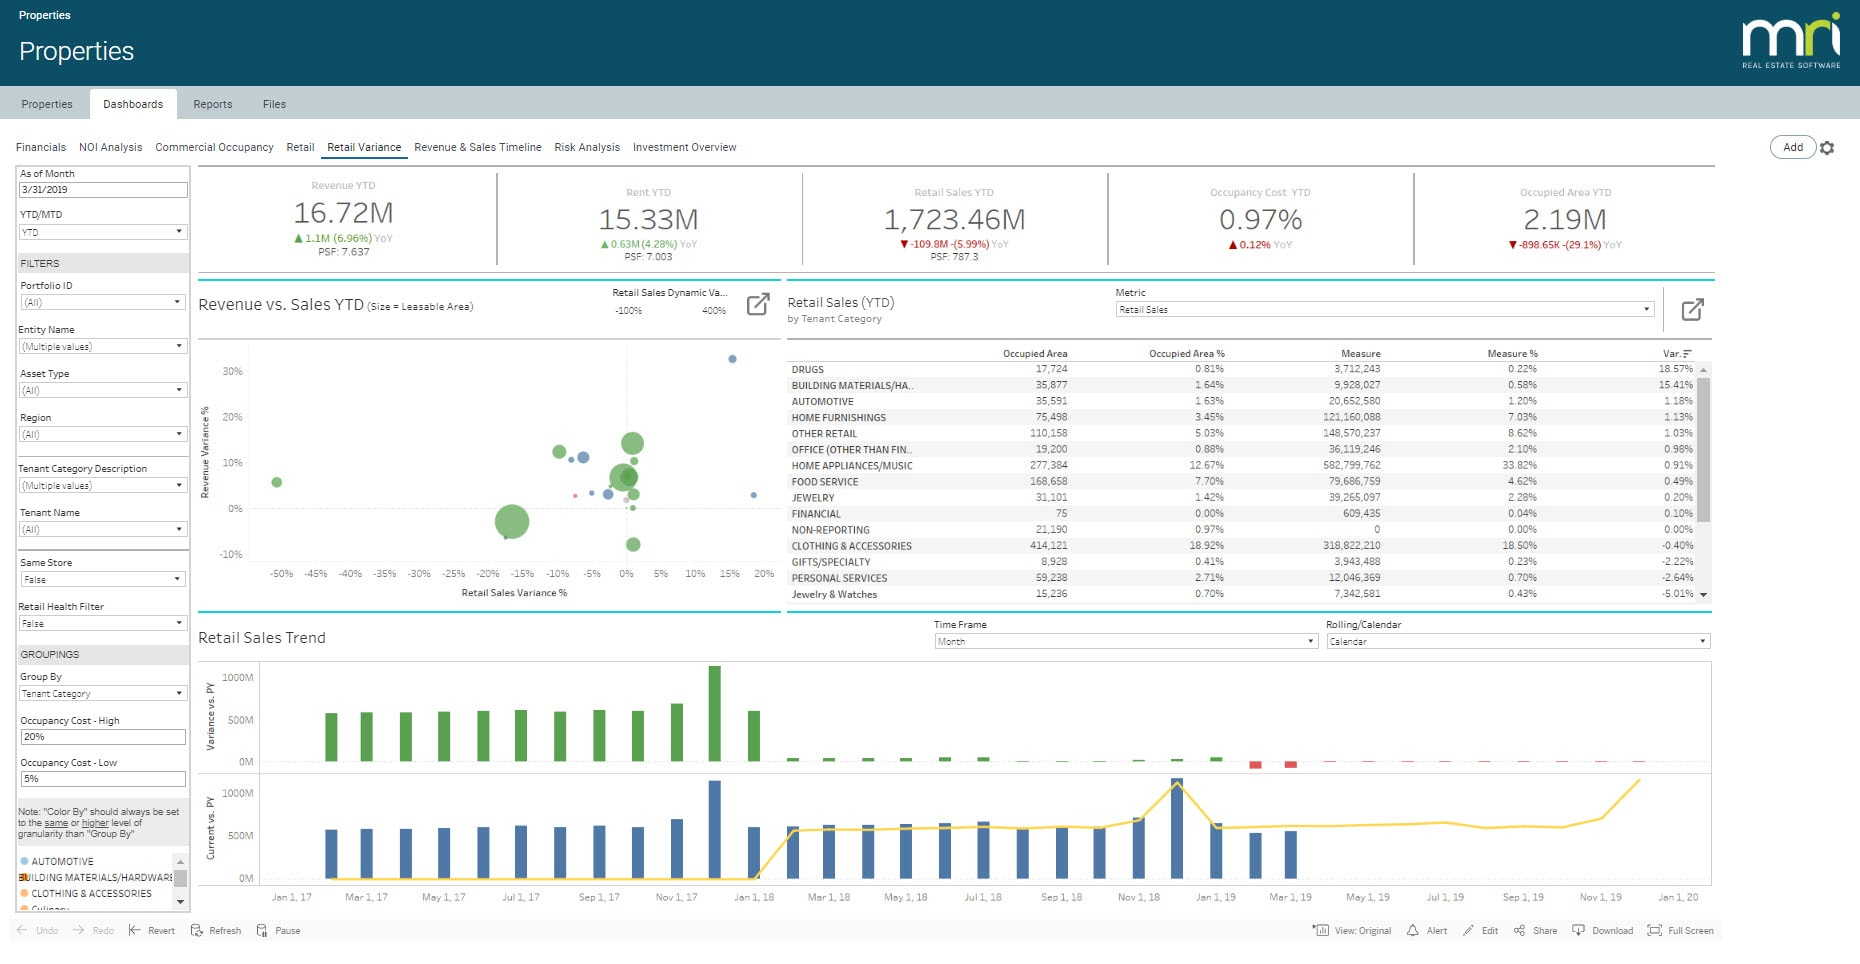
\includegraphics[width=0.99\linewidth]{assets/mri-workplace-central-demo.jpg}
    \caption{Интерфейс программы \textit{MRI Workplace Central}}
    \label{fig:mri-workplace-central-demo}
\end{figure}

\subsubsection{Платформа \textit{Envoy} }
\label{ssub:domain:solution-overview:envoy}

является популярным решением для управления рабочими местами, помещениями и посетителями, которая помогает компаниям организовать гибридную работу, оптимизировать использование офисных ресурсов и улучшить взаимодействие между сотрудниками.

Система \textit{Envoy} предоставляет удобные инструменты для бронирования рабочих мест и комнат для встреч. Одной из ключевых особенностей \textit{Envoy} является функция управления посетителями, которая позволяет регистрировать гостей, выдавать пропуски и уведомлять сотрудников о прибытии посетителей. Однако в сравнении с \textit{MRI Workplace Central}, \textit{Envoy} предлагает меньше функций для управления активами и оборудованием, что может быть недостатком для компаний, которым требуется комплексное решение для управления всеми офисными ресурсами.

Интеграция с внешними системами, а именно: календарными системами \textit{Google Calendar} и \textit{Microsoft Outlook}, системами контроля доступа, такими как \textit{Kastle} и \textit{Brivo}, что упрощает управление доступом сотрудников и посетителей в помещения. Кроме того, \textit{Envoy} предлагает \textit{REST API} для интеграции с другими корпоративными системами. Однако, несмотря на широкие возможности интеграции, некоторые компании могут столкнуться с ограничениями в настройке системы под свои нужды, особенно если требуется сложная интеграция с внутренними системами.

Возможности платформы \textit{Envoy} включают:

\begin{itemize}
    \item предварительную проверку состояния здоровья сотрудников и гостей с помощью интеграции форм самодиагностики;
    \item управление графиком присутствия сотрудников в офисе в рамках гибридной модели работы (например, настройка «кто когда работает из офиса»);
    \item отслеживание плотности заполняемости помещений для соблюдения санитарных норм и социального дистанцирования;
    \item автоматическое создание цифровых журналов посещений без необходимости ручной регистрации;
    \item настройку правил доступа в зависимости от условий (например, разрешён вход только после подтверждения условий пребывания);
    \item встроенные сценарии на случай инцидентов (эвакуация, проверка безопасности, учёт присутствующих в здании);
    \item поддержку \textit{SSO} (\textit{Single Sign-On}) для корпоративных пользователей через \textit{Okta}, \textit{Azure AD} и другие провайдеры;
    \item интеграцию с системами уведомлений и мессенджерами (например, \textit{Slack}, \textit{MS Teams}) для информирования в реальном времени;
    \item уведомления при прибытии курьеров, доставок и других внешних лиц в офис;
    \item гибкую настройку политик безопасности в зависимости от ролей, офисов, дней недели или специфики событий.
\end{itemize}

Платформа \textit{Envoy} уделяет большое внимание безопасности, предлагая многофакторную аутентификацию для повышения защиты доступа к системе. Управление правами доступа на основе ролей сотрудников позволяет контролировать, кто и какие функции системы может использовать. Все данные передаются и хранятся в зашифрованном виде, что соответствует современным стандартам безопасности, таким как \textit{GDPR}~\cite{web_gdpr}. Система также ведет журнал всех действий пользователей, что позволяет проводить аудит и мониторинг подозрительной активности~\cite{web_envoy_employee_data}. Однако, несмотря на высокий уровень безопасности, некоторые компании могут столкнуться с ограничениями в настройке политик безопасности, особенно если требуется сложная конфигурация. Процесс работы в \textit{Envoy} показан на рисунке~\ref{fig:envoy-demo}.

\begin{figure}[h]
\centering
    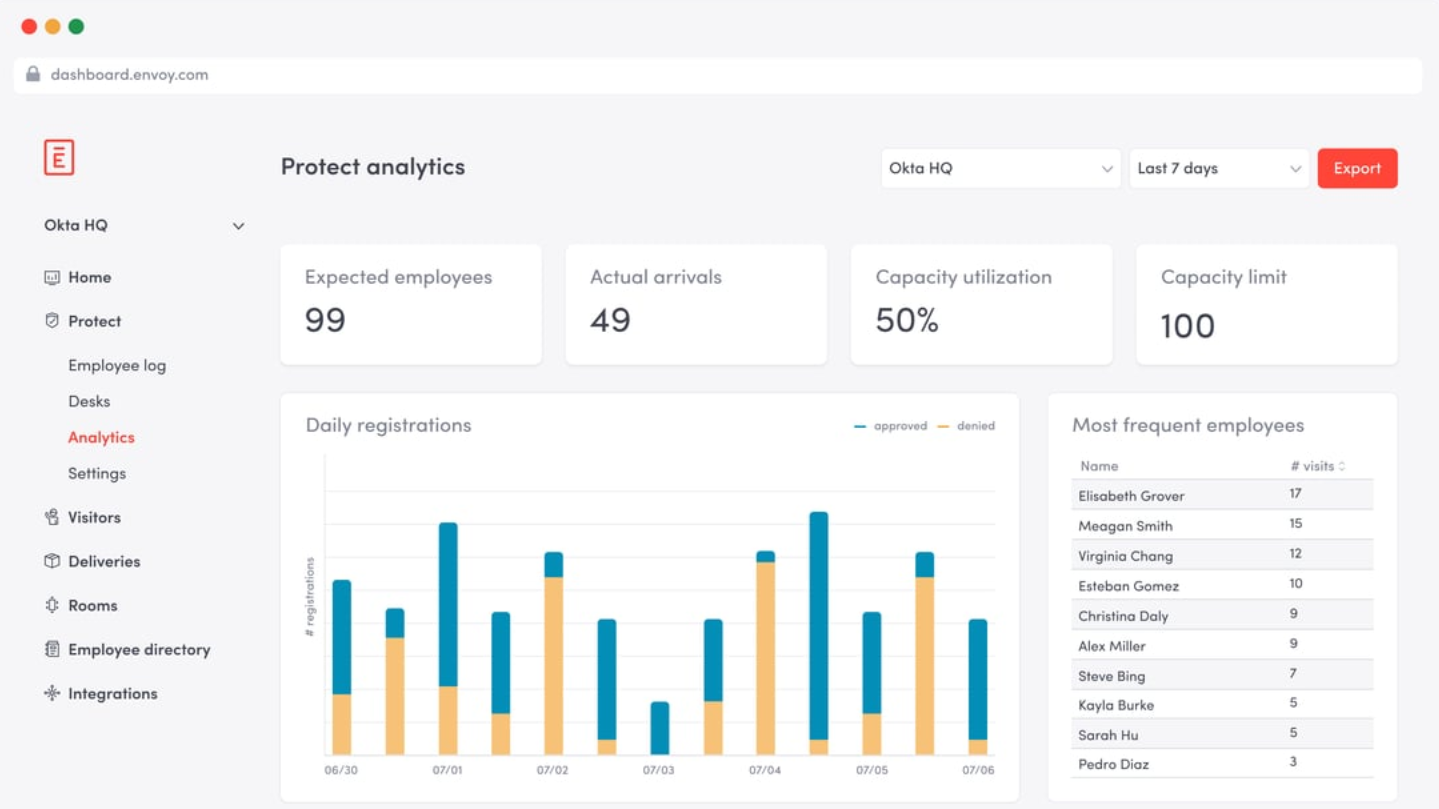
\includegraphics[width=0.99\linewidth]{assets/envoy-demo.png}
    \caption{Интерфейс платформы \textit{Envoy}}
    \label{fig:envoy-demo}
\end{figure}


Рассмотренные темы охватывают ключевые аспекты организации офисных помещений, их автоматизации и существующих решений для управления рабочими местами и ресурсами. Был проведен анализ различных методов управления офисными информационными процессами, выявлены их преимущества и недостатки, а также рассмотрены специализированные системы, такие как \textit{MRI Workplace Central} и \textit{Envoy}. Эти исследования демонстрируют, что современные офисные информационные системы значительно повышают эффективность работы, обеспечивают гибкость управления пространствами и улучшают взаимодействие сотрудников. В конечном итоге, внедрение автоматизированных решений способствует оптимизации бизнес-процессов, снижению операционных издержек и повышению конкурентоспособности компаний в условиях динамичного рынка.
